\chapter{Methodology} % Main chapter title

\label{Methodology} % For referencing the chapter elsewhere, use \ref{Chapter2}

\section{Dataset Evaluation}
\label{sec:datasets}

\begin{marginfigure}[] % move figure up by 1 line -5\baselineskip
    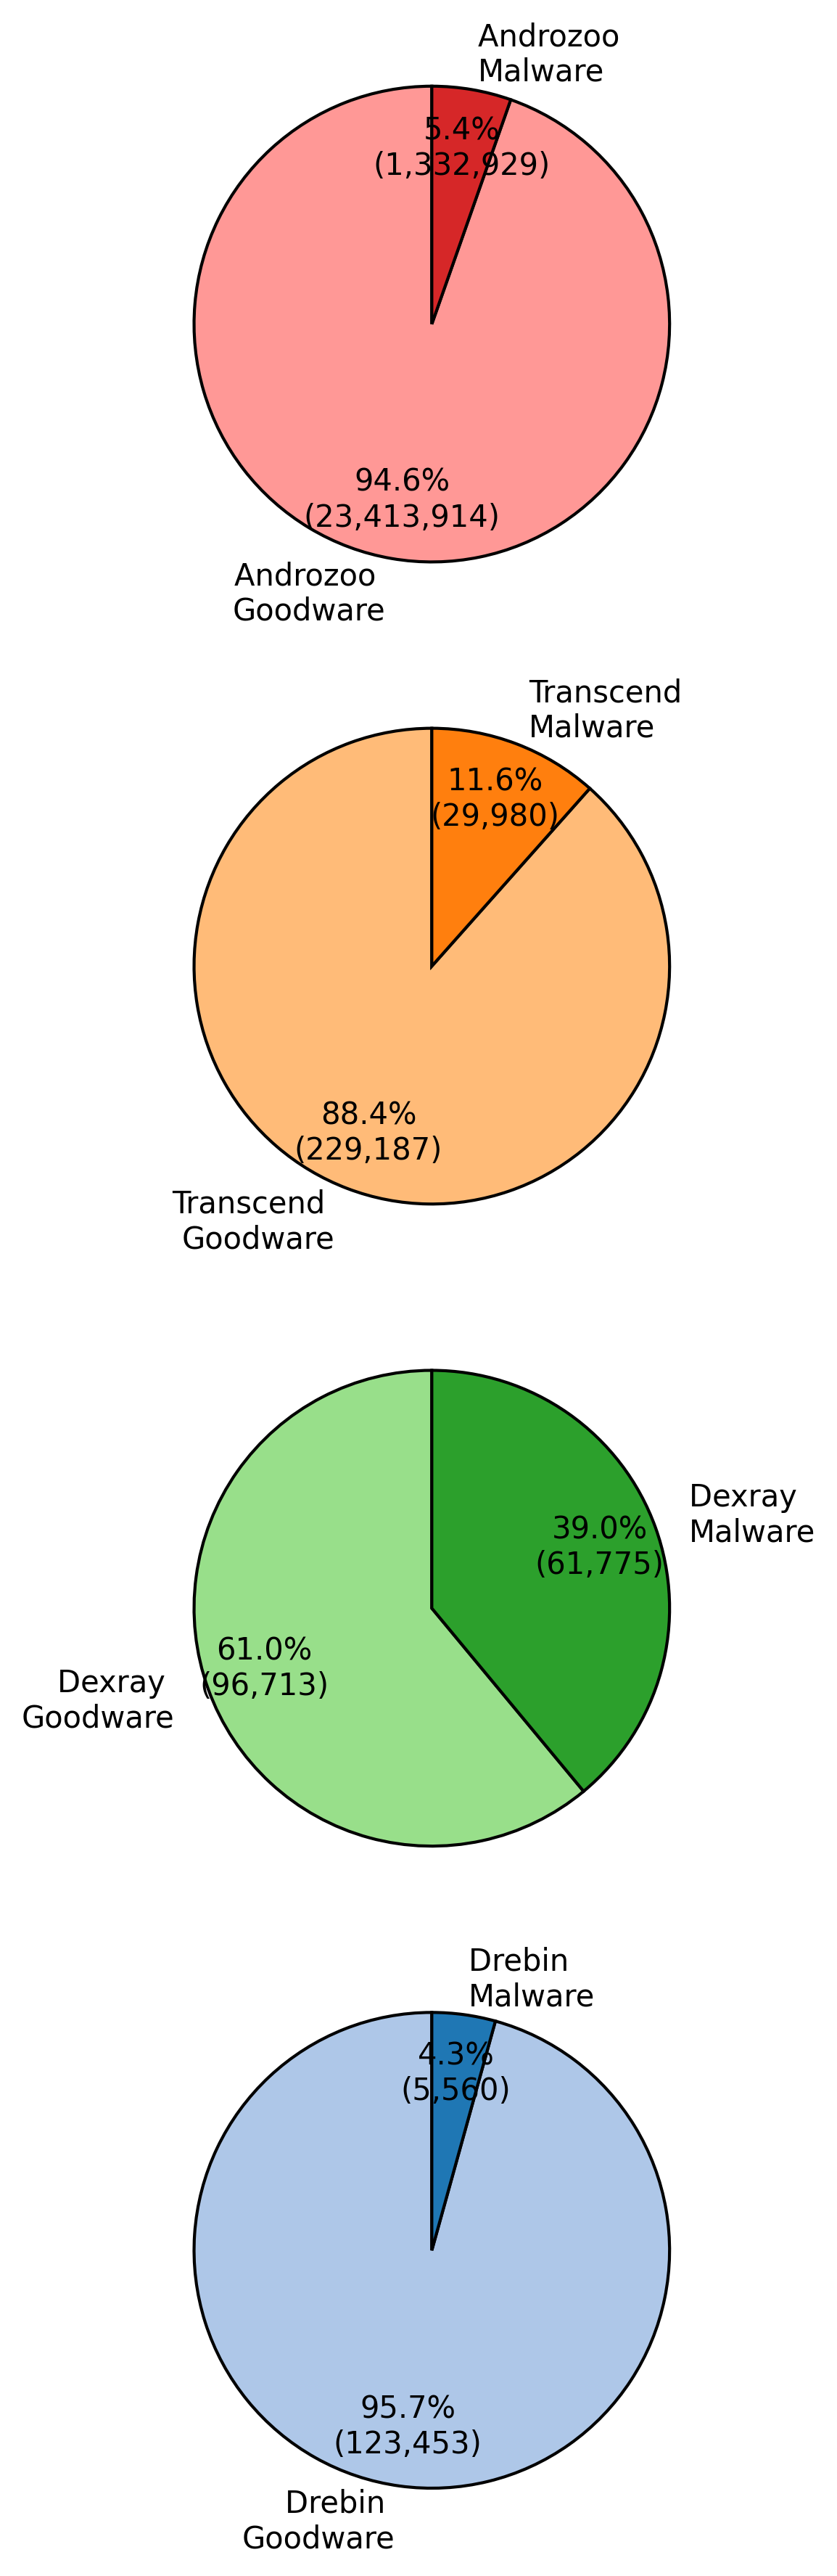
\includegraphics[width=1\marginparwidth]{3_Methodology/malware_goodware_ratios.png}
    \caption{\label{fig:malratios}
    Distribution of malware and goodware samples across datasets shown as pie charts.
    The datasets analyzed are are ordered by size from largest to smallest.
    The number of APKs contained in the Dataset are shown in brackets}
\end{marginfigure}

The evaluation of datasets forms a critical foundation for the success of any machine learning task, 
especially in security sensitive applications such as mobile malware detection. 
A robust dataset not only enables effective training of models but also ensures generalizability 
across various scenarios, including concept drift. 
This section outlines the dataset evaluation process undertaken for this research.

The datasets that are evaluated are introduced in subsection \ref{sec:amd}.
The Drebin, Transcend, and DexRay datasets are well suited for comparison because they are 
specifically designed to serve as benchmarks for training and evaluating models on android malware detection. 
Each dataset is designed to train specific models and assess their performance. 
Androzoo is notably different because it serves as a large repository for Android APKs rather 
than a closed dataset specifically designed for training and benchmarking algorithms. 
Additionally, it is continuously updated and expanded by the authors.

When comparing the number of APKs of each dataset, Androzoo has the most APKs with 25,059,602 
(as of 06.103.2025 14:23). 
Since it is a repository, it will continue to grow larger.
The biggest of the benchmarking datasets is Transcend, which has 259,230 available APKs. 
This is followed by DexRay with 159,803 APKs, and then Drebin with 129,013 APKs. 
In general, larger datasets are better for training and evaluating a model. 
However, this is only true if the dataset size correlates with novelty, 
meaning it introduces unique and diverse cases. 
For example, a dataset containing applications from various time periods or regions 
ensures that the model can generalize to unseen scenarios. 
This has been shown by \cite{scalinglaws}, 
where they demonstrated that the performance of Transformer Decoder Models 
correlates with the size of the data used to train them.

Figure \ref{fig:malratios} shows the label distribution for each dataset. 
Notably, the DexRay dataset has an unusually high percentage of malware APKs. 
On one hand, this could help the model learn more diverse representations of malicious APKs. 
On the other hand, Arp et al. refer to this as a sampling bias, where 
"the collected data does not adequately represent the true distribution of 
the underlying security problem" \cite{dodo}. 
While the actual label distribution is unknown 
(and likely changes depending on the models use case), 
it seems unlikely that 39\% of APKs are generally malware. 
Similarly, the Transcend dataset also has a high malware rate, 
with over 10\% of its samples being malicious. 
In comparison, Androzoo and Drebin show about 5\% malware APKs in their distributions. 
The Androzoo Malware labels were derived from 
virustotal\footnote{https://www.virustotal.com/gui/home/upload} by 
Euphony \cite{androzoo_malware} in 2017, 
which means that they are outdated as newer APKs were not evaluated.

%\vspace*{-2\baselineskip} % Move the figure upwards
\begin{marginfigure}[-50pt] % 't' specifies top placement
    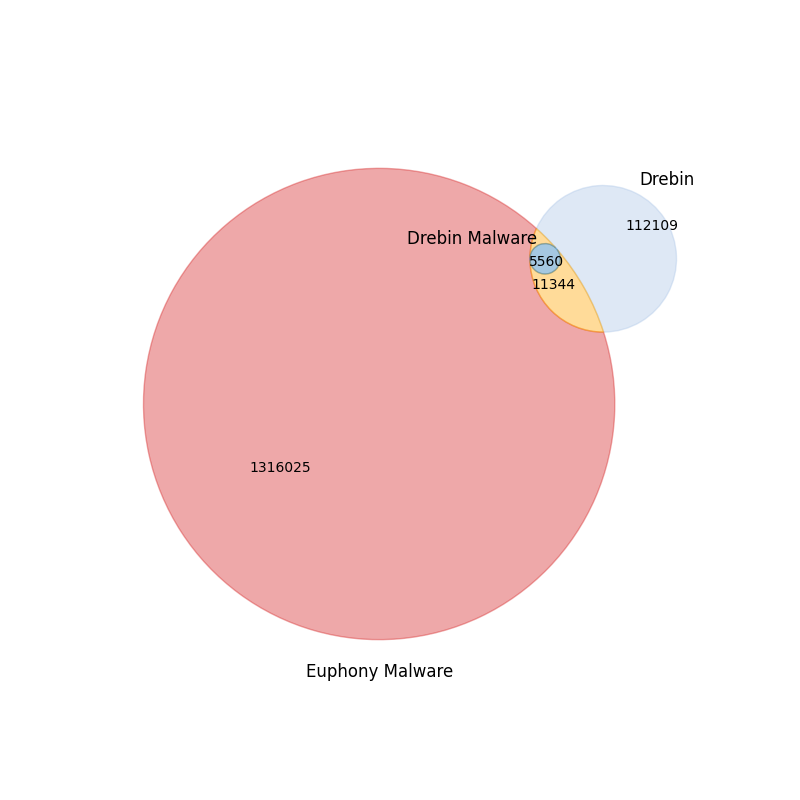
\includegraphics[width=1\marginparwidth]{3_Methodology/euphony_drebin_overlap.png}
    \caption{\label{fig:euphony_drebin_overlap}
    Overlap between the Drebin and Euphony datasets. 
    The light blue circle represents Drebin, where 112,109 APKs are classified as goodware (excluding overlap).
    The red circle represents Euphony, which contains 1,316,025 APKs labeled as malware (excluding overlap). 
    The dark blue circle represent those 5560 APKs, that are considered malware for both Drebin and Euphony.
    The intersection in orange highlights 11,344 APKs classified as goodware by Drebin but as malware by Euphony.}
\end{marginfigure}

One important aspect is that there is no clear definition of malware, 
which significantly impacts the analysis. 
This lack of a universal definition leads to inconsistencies in classification across datasets, 
making it challenging to validate labels and draw reliable comparisons. 
Without a standardized framework, each dataset might apply its own criteria.
Each dataset can have different interpretations of what is considered malware, 
often based on criteria such as the presence of specific permissions, 
API calls, or behaviors flagged by antivirus software. 
One dataset might classify an APK as malware due to aggressive adware practices, 
while another might only consider code executing malicious payloads. 
These differences make the validation of labels very difficult.
One Example that shows this issue is evident when comparing Drebin with Euphony 
(figure: \ref{fig:euphony_drebin_overlap}).
Euphony and Drebin have a common subset, none of the sets is a true subset of the other.
However, the APKs labeled as malware by Drebin are a true subset of Euphony.
Additionally, Euphony classifies multiple APKs as malware that were classified as goodware by Drebin.
The fact that there are no APKs that are classified as malware by Drebin and Goodware 
by Euphony shows that Drebin applies a more narrow definition on what is considered malware.
Further Overlaps of different Datasets are visualized in the Appendix 
(figure: \ref{fig:dataset_overlap}).

\subsection{Temporal Evaluation}

\begin{figure*}[b]
    \centering
    \begin{minipage}{1.5\textwidth}
        \centering
        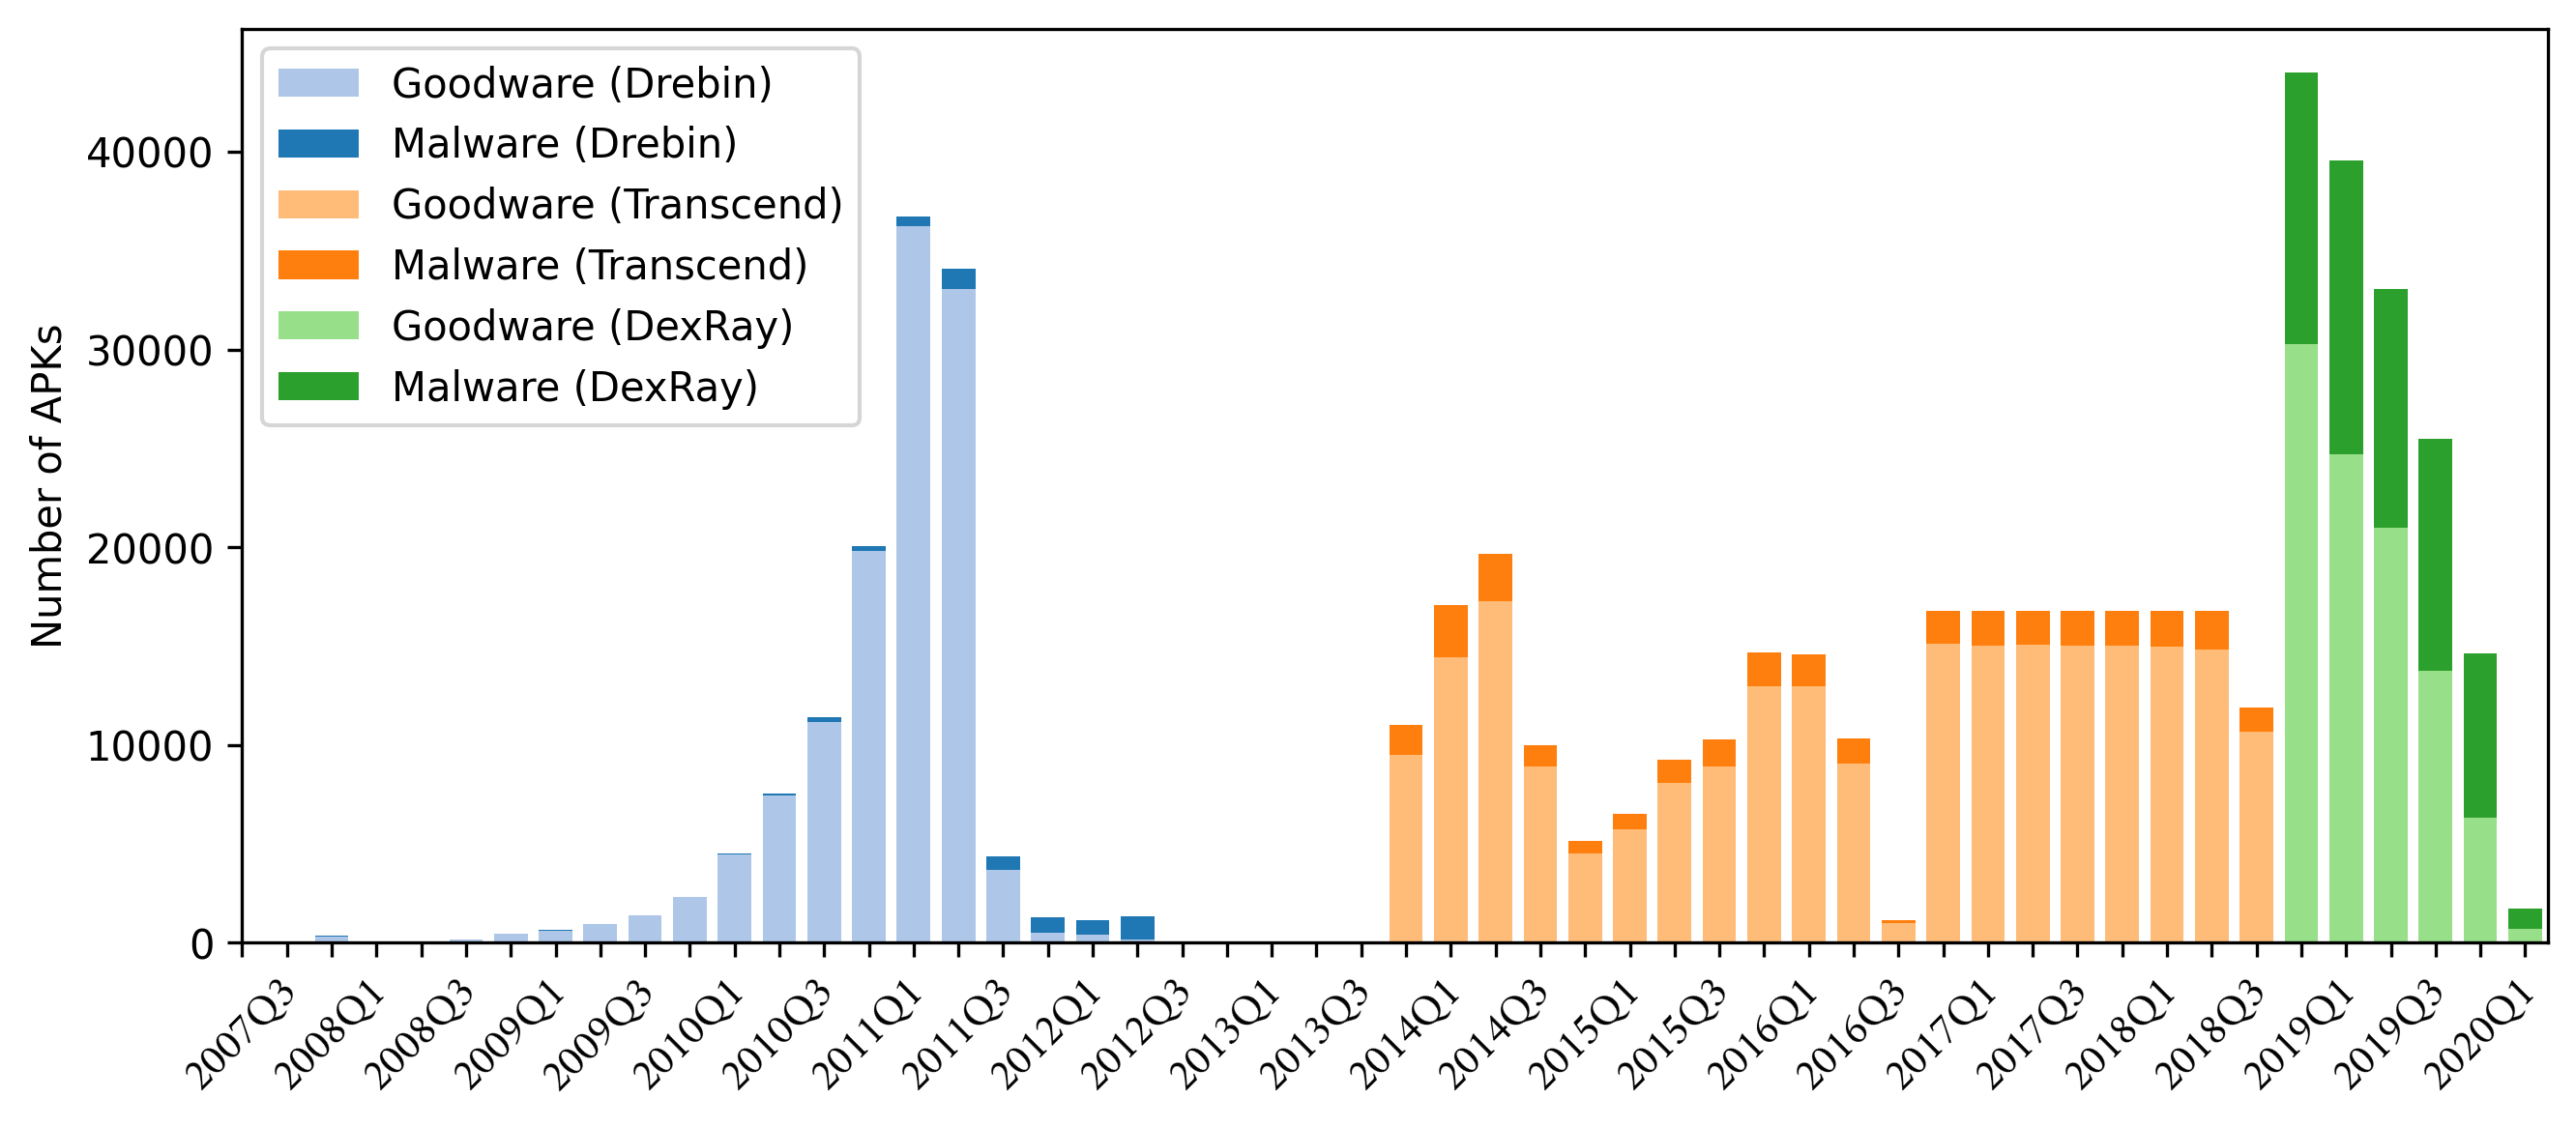
\includegraphics[width=\textwidth]{3_Methodology/dataset_time_distribution.png}
        \captionsetup{width=\textwidth}
        \caption{\label{fig:dataset_time_evaluation}
        Temporal distribution of Android APKs across three datasets (Drebin, Transcend, and DexRay), 
        categorized into goodware and malware.
        The Data is derived from metadata of the classes.dex file of each APK.
        }
    \end{minipage}
\end{figure*}

The temporal evaluation of APKs is often based on metadata of the classes.dex component, 
as it contains crucial timestamp information reflecting the compilation date of the code. 
This metadata serves as a reliable indicator of the APKs development period, 
providing a foundation for chronological analyses.
While this often works (figure: \ref{fig:dataset_time_evaluation}), 
it becomes more common that this meta information is not available. 
This lack of metadata poses challenges for temporal evaluation, 
as it limits the ability to analyze trends and shifts in malware development over time, 
as seen by the temporal evaluation of the androzoo repository 
(figure: \ref{fig:androzoo_temporal}).

The distribution of the .dex dates of the three datasets 
(figure: \ref{fig:dataset_time_evaluation}) shows that the datasets are in succession of one another. 
There is no temporal overlap, which explains why there is no APK present in more than one of 
these datasets (figure: \ref{fig:dataset_overlap}). 
There is a gap between the third quarters of 2012 and 2013 where neither dataset has samples. 

While the Transcend Dataset seems to be evenly distributed, 
the other two datasets seem to show varying volumes over time. 
This holds true for the overall volume but also about the evenness of the label distribution. 
Here Drebin and DexRay show unbalanced malware sample behavior. 
This uneven distribution can affect the generalizability of findings.

% (Extendable)
One Example where concept drift is visible is, 
that the size of packaged APKs grows with time \ref{fig:dataset_size_evaluation}.
The three datasets show different distributions of APK sizes, 
where Drebin shows the smallest and DexRay the biggest APKs on average.
The Plot also shows that the labels of all datasets are more evenly distributed by the APK size, 
compared to the .dex date of the APK.

% Nochmal Drüberlsesen:::!!!
When evaluating a model regarding the concept drift of malware, 
the Transcend dataset shows the most potential.
However, only considering one dataset limits the generalizability of an approach, 
so the evaluation on multiple datasets is even better.
One Problem is, that all three datasets only contain APKs where the .dex date is available.
The temporal evaluation of Androzoo \ref{fig:androzoo_temporal} showed that this is for most 
modern APKs not the case.
It follows that each of the datasets are Biased in their selection of APKs and are 
therefore not fit for representing the True APK landscape. 

\begin{figure*}[b!]
    \centering
    \begin{minipage}{1.5\textwidth}
        \centering
        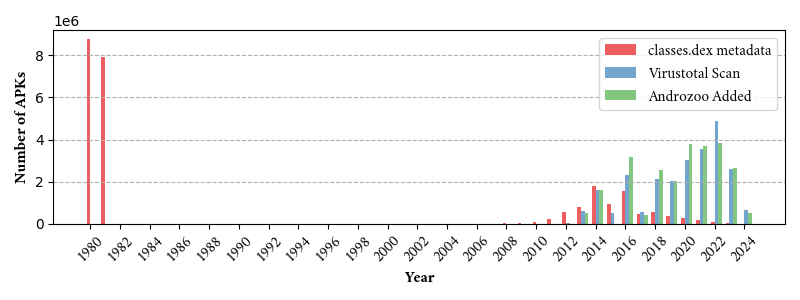
\includegraphics[width=\textwidth]{A_Images/androzoo_temporal.png}
        \captionsetup{width=\textwidth}
        \caption{\label{fig:androzoo_temporal}
        Temporal distribution of APKs based on three key attributes: 
        classes.dex metadata, Virustotal Scan, and Androzoo Added. 
        The red bars (classes.dex metadata) show a large spike in 1980 to 1982, 
        likely due to incorrect or missing metadata values. 
        The blue (year of first scan by virustotal on that APK) and 
        green (year this APK was added to the androzoo repository) bars 
        indicate a consistent increase in APK activity from 2010 onward, 
        peaking around 2020 to 2022, reflecting the growing adoption of Android 
        and corresponding malware collection efforts. 
        The discrepancies between attributes highlight potential issues in 
        dataset metadata accuracy and consistency.
        }
    \end{minipage}
\end{figure*}


\newpage

\subsection{Code Evaluation}

When checking for Malware, an important representation of an APK is its code.
As the code describes the logic of what the App does, it seems logical that, if the 
code is sufficiently evaluated, the harmfulness of the APK can be derived.
Especially Transformer models show promise in interpreting the code of an APK as they work very well as LLMs.

It follows that not just time distributions of the datasets should be evaluated, but also the distribution of code.
There are two major ways of decompiling an APK into a code representation.
The classes.dex file can either be decompiled into Java code or into lower level Smali code.

For the decompilation of the APK into Java code, dex2jar\footnote{https://github.com/pxb1988/dex2jar} is first used to decompile the classes.dex file into a JAR file.
The JAR file can then be further decompiled into plain Java code. 
The resulting Java code is on the one hand easy to interpret due to its higher level nature, 
however the decompiled code is prone to obfuscation that can make it hard to interpret.
One example on how obfuscation can make the logic of the App more complex is by changing the package names, 
so that it is not possible to see the entry points that are defined in the Manifest file. 
This phenomenon is further evaluated in tables \ref{tab:matching_java_classes_transcend} and \ref{tab:matching_java_classes_dexray} in section
\ref{sec:tran_enc}.

There also is an option to decompile the classes.dex file into Smali code.
Smali is the human readable representation of the Dalvik bytecode that is found in the raw classes.dex file.
Smalie therefore is to Dalvik bytecode, what Assambly is to machine code.
The Smali representation of an APK can be retrieved by using Apktool\footnote{https://apktool.org/} on the classes.dex file.
While the Smali representation is more accurate the original bytecode and also is more robust to obfuscation, 
the readability is much harder due to the lower level and niche nature.

\begin{figure*}[b!]
    \centering
    \begin{minipage}{1.5\textwidth}
        \centering
        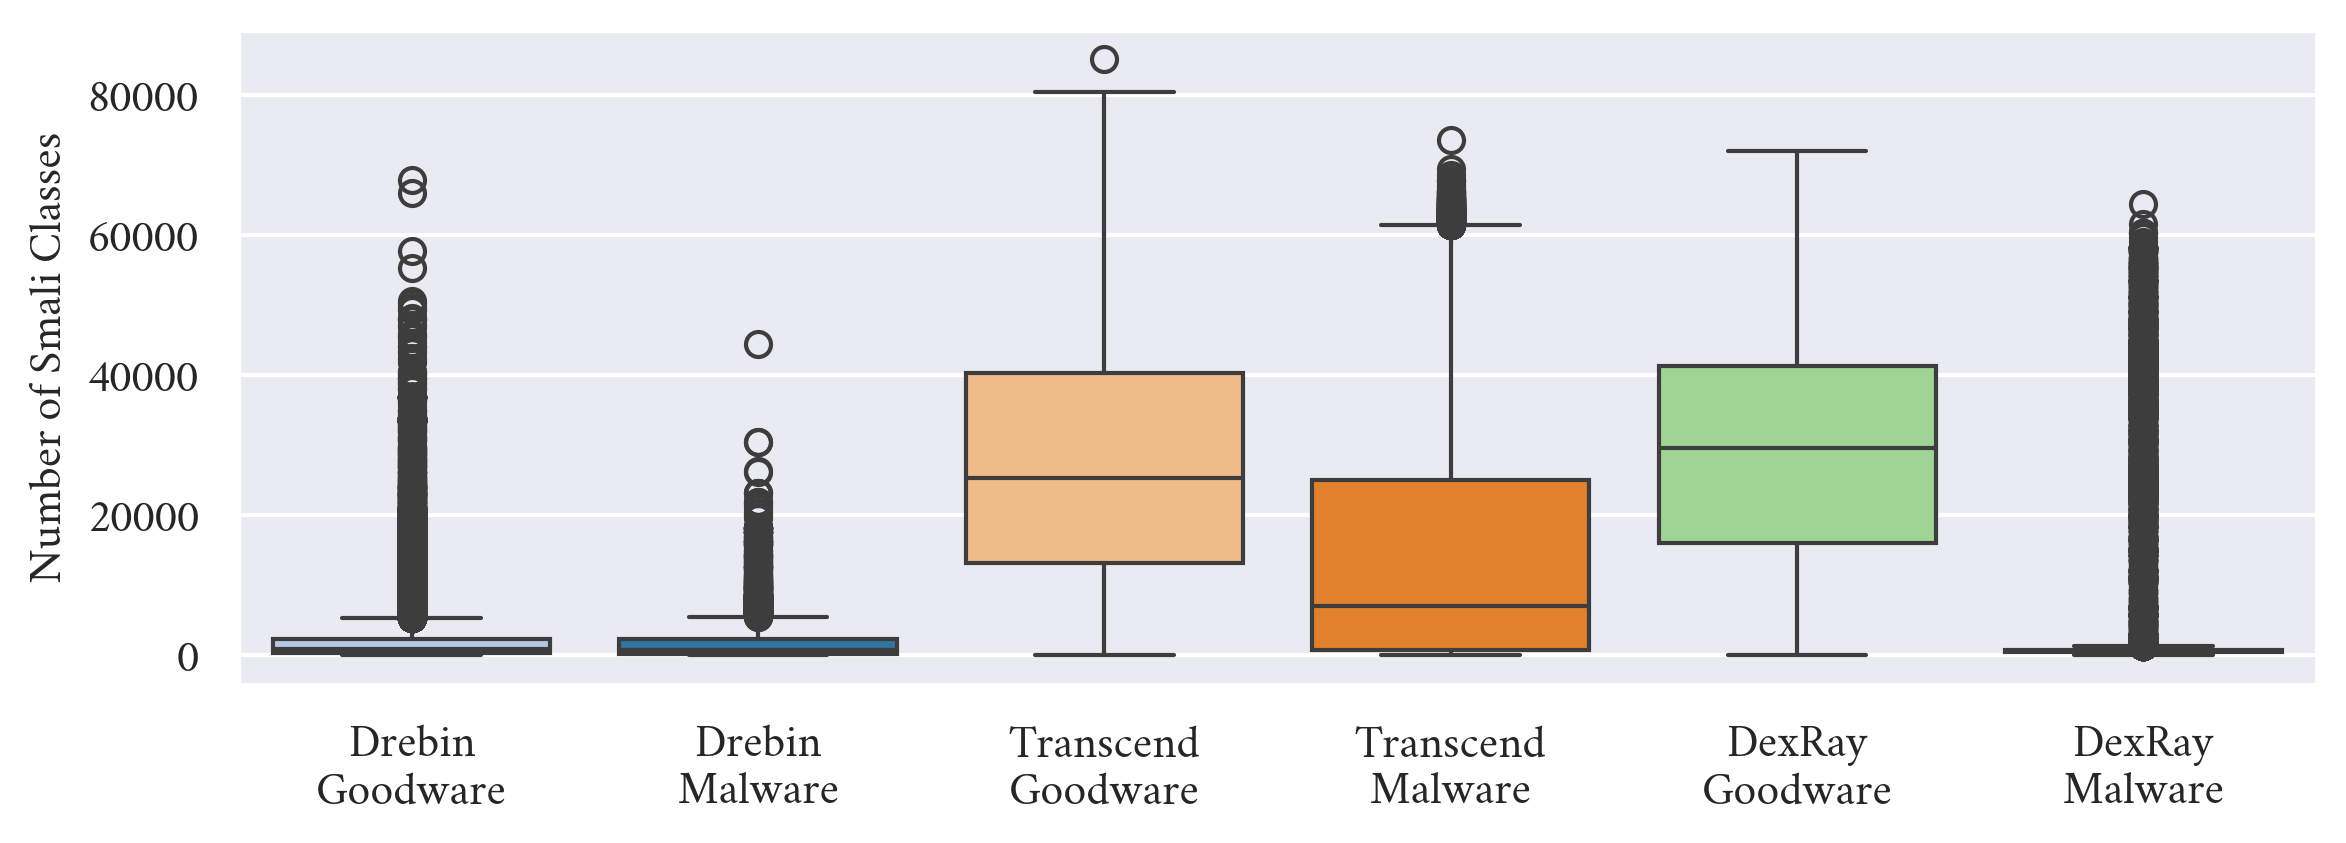
\includegraphics[width=\textwidth]{3_Methodology/smali_class_boxplots.png}
        \captionsetup{width=\textwidth}
        \caption{\label{fig:smali_class_boxplots}
        The boxplot shows the distribution of Smali classes in Android apps 
        across the Drebin, Transcend, and DexRay datasets, 
        split into Goodware and Malware. 
        Drebin and Transcend have an similar Smali class distribution 
        between Goodware and Malware.
        The DexRay Dataset shows a high inbalance in the number of Smali classes 
        between the two labels.
        }
    \end{minipage}
\end{figure*}

\newpage

\begin{margintable}[1\baselineskip] % Move table down by 1 line
    \caption{\label{tab:smali_distribution}Smali Statistics Summary for DexRay, Transcend, and Drebin.}
    \footnotesize
    \begin{tabular}{@{}lccc@{}}
        \toprule
        \tabhead{Label} & \tabhead{Q1} & \tabhead{Median} & \tabhead{Q3} \\
        \midrule
        \multicolumn{4}{l}{\textbf{DexRay}} \\
        Goodware & 16106 & 29546 & 41352 \\
        Malware & 445 & 598 & 817 \\
        \midrule
        \multicolumn{4}{l}{\textbf{Transcend}} \\
        Goodware & 13145 & 25364 & 40372 \\
        Malware & 764 & 7057 & 25015 \\
        \midrule
        \multicolumn{4}{l}{\textbf{Drebin}} \\
        Goodware & 331 & 901 & 2353 \\
        Malware & 173 & 805 & 2316 \\
        \bottomrule
    \end{tabular}
\end{margintable}

As part of the code evaluation of this thesis, 
the same three datasets as in the time evaluation were considered.
For each APK of the datasets, the classes.dex file was decompiled 
in both an Java and an Smali code representations.
The code representation of an APK is quite complex and only hardly allows 
statistical aalysis.
One approach that was possible is to count the classes of the code representations for each APK,
reducing the complexity from a repository per app to a number.
Figure \ref{fig:smali_class_boxplots} shows the Boxplots of the distribution 
of Smali classes of the apps in the dataset distinguishing 
between the label of the APK.
The Boxplots show, that Drebin has a generally low amount of Smali classes 
per APK, wich can be explained by the Apps being 
older (as shown in table \ref{fig:dataset_time_evaluation}) and 
smaller (as shown in table \ref{fig:dataset_size_evaluation}) than those of the other datasets.

A second observation, is that the DexRay Dataset is highly inbalanced.
This is apparent both from the Boxplot (figure \ref{fig:smali_class_boxplots}) and also by table \ref{tab:smali_distribution},
that quantifies the distribution of smali classes by computing the Q1, Median and Q3 values of each of the Datasets.
When looking further into \ref{tab:smali_distribution} the issue becomes even more apparent. 
Q1, Median and Q3 differ between the labels by a factor of 35-50, this makes any approach that makes label 
predictions based on Smali code of that dataset questionable (for example \cite{dexbert,detectbert,dexray}).

\begin{margintable}[1\baselineskip] % Move table down by 1 line
    \caption{\label{tab:java_distribution}Java Statistics Summary for Drebin, Transcend, and DexRay.}
    \footnotesize
    \begin{tabular}{@{}lccc@{}}
        \toprule
        \tabhead{Label} & \tabhead{Q1} & \tabhead{Median} & \tabhead{Q3} \\
        \midrule
        \multicolumn{4}{l}{\textbf{Drebin}} \\
        Goodware & 19 & 60 & 176 \\
        Malware & 18 & 66 & 224 \\
        \midrule
        \multicolumn{4}{l}{\textbf{Transcend}} \\
        Goodware & 854 & 1800 & 2899 \\
        Malware & 52 & 738 & 2244 \\
        \midrule
        \multicolumn{4}{l}{\textbf{DexRay}} \\
        Goodware & 1035 & 2007 & 3084 \\
        Malware & 7 & 11 & 11 \\
        \bottomrule
    \end{tabular}
\end{margintable}


The Transcend dataset shows less inbalance in code volume compared to the DexRay dataset.
Especially on Q1 differs by a factor of 17,2 showing that there are relatively more code sparse Malware than Goodware APKs.
When comparing the upper end of the spectrum, the inbalance becomes less drastic with an factor of ~3,5 for the median and 1,6 for the Q3.
Drebin shows overall a very good inbetween class balance of Smali classes when compared to the other datasets.

The decompilation into Java classes paints a similar picture. 
For comparison there is a similarly structured table showing the statistical properties of the Java class distribution \ref{tab:java_distribution}.
Additionally in the Appendix (\ref{sec:appendiximages}) there is another Boxplot \ref{fig:java_class_boxplots} that has the same 
structure as figure \ref{fig:smali_class_boxplots}.
When evaluating the volume of Java and Smali classes over all datasets a correlation coefficient of 0.92 proofs that they are very similar.

Table \ref{tab:java_distribution} shows that for the DexRay Dataset, more than 75\% of the malware APKs have less than 12 Java classes, 
while 75\%  of the goodware labeled ones have more than 1000 Java classes.
This makes it highly likely that an classifier will just differentiate 
between the number of classes present and derive the prediction from this information.
This leads to the conclusion, that the DexRay dataset is generally insufficient for training a code based classifier.


\section{Baseline Creation}
\label{sec:baseline}

When generating a baseline for mobile malware detection, concept drift hast to be considered.
Jordaney et al. \cite{transcend} showed that there is a concept drift for android malware.
In order to train a model that is robust again this concept drift, 
Kan et al. \cite{tesseract} propose to split the data into train and test data in a particular way.
The training data should be from before the test data, 
while keeping the same label ratio in between splits.  
The reason for this is to make sure that the model does not train on features of the data, 
that are prone to concept drift.
The punishment for this is maximized if the train and test data is sequential.
In order to account for and validate the concept drift in the domain of malware detection,
the following baselines where both created on a dataset that is split randomly into train and test subsets
and also split time based as proposed by \cite{transcend}.
The data is split into 80\% test and 20\% train data for both splitting Approaches.
The evaluation is always done in a balanced manner, penalizing mistakes on the less frequent malware label more.

\subsection{Non Transformer Approaches}

\begin{table*}[t!]
    \begin{minipage}{1.5\textwidth}
        \captionsetup{width=\textwidth}
        \caption{\label{tab:treestump} Tree Stump (balanced class weights) results by dataset, feature, and split.}
    \end{minipage}
    \small
    {\renewcommand{\arraystretch}{1.5} % Increase row height for better readability
        \begin{tabularx}{\linewidth}{@{}l l l r r r r r@{}} % Adjusted alignment: l for text, r for numbers
            \toprule
            \textbf{Dataset} & \textbf{Feature} & \textbf{Split} & \textbf{Accuracy} & \textbf{Precision} & \textbf{Recall} & \textbf{F1 Score} & \textbf{Threshold} \\
            \midrule
            Drebin & Java classes & random     & 10.16\% & 4.40\% & 99.07\% & 8.43\% & 2.5 \\
                   & Java classes & time based & 7.39\%  & 4.31\% & 96.49\% & 8.24\% & 3.5 \\
                   & Smali classes & random    & 76.01\% & 6.14\% & 33.24\% & 10.37\% & 247.5 \\
                   & Smali classes & time based & 7.15\%  & 4.31\% & 96.76\% & 8.24\% & 33.5 \\
                   & APK size     & random     & 10.94\% & 4.32\% & 96.10\% & 8.27\% & 59676 \\
                   & APK size & time based & 6.62\%  & 4.35\% & 98.38\% & 8.33\% & 59676 \\
            \midrule
            Transcend & Java classes & random     & 90.05\% & 70.58\% & 23.38\% & 35.12\% & 17.5 \\
                         & Java classes & time based & 82.63\% & 36.58\% & 68.35\% & 47.65\% & 967.5 \\
                         & Smali classes & random    & 77.63\% & 27.44\% & 57.28\% & 37.10\% & 9699.5 \\
                         & Smali classes & time based & 77.61\% & 31.23\% & 77.85\% & 44.58\% & 15101.5 \\
                         & APK size     & random     & 18.75\% & 11.90\% & 94.56\% & 21.14\% & 57904190 \\
                         & APK size & time based & 39.27\% & 11.77\% & 65.44\% & 19.96\% & 11054373 \\
            \midrule
            DexRay & Java classes & random     & 92.05\% & 93.04\% & 86.37\% & 89.58\% & 90.5 \\
                   & Java classes & time based & 94.74\% & 89.67\% & 97.65\% & 93.49\% & 90.5 \\
                   & Smali classes & random    & 92.10\% & 93.19\% & 86.36\% & 89.64\% & 1395.5 \\
                   & Smali classes & time based & 94.59\% & 89.35\% & 97.63\% & 93.31\% & 1395.5 \\
                   & APK size     & random     & 48.53\% & 42.97\% & 91.97\% & 58.58\% & 79432704 \\
                   & APK size & time based & 44.78\% & 39.11\% & 76.98\% & 51.87\% & 67843648 \\
            \bottomrule
        \end{tabularx}
    }
\end{table*}

A very simple classifier is a decision tree stump.
This stump is infering a threshold based on the training data and then using it to predict a label for new samples.
To make it even simpler for creating a first baseline, in Table \ref{tab:treestump} only one feature is considered when calculating the tree stump.
The table shows how the Drebin dataset is most robust to this very basic approach.
For Drebin, neither of the considered features (Number of Java classes, Number of Smali classes \& Size of the packaged APK)
is fit for successfully separating the labels with one threshold.
On the first glance it seems unlikely, that the thresholds for the APK sizes are constant over both different dataset splits.
Since the threshold is changing for some other random splits (by using other random seeds),
this phenomenon seems to be due to chance.
This can be explained by how the threshold is derived from the training data
using the gini coefficient \cite{gini}.

On the Transcend dataset, the Tree Stump approach achieve better results.
Here the concept drift can be observed by the changing thresholds between the split methods.

The most shocking result is, that the DexRay dataset can be solved with an F1 score of 93,49\% 
with a simple Tree stump approach on the Java classes feature.
This shows how inbalanced the dataset is and how it is unfit for evaluatig models 
that rely on code based features.
Another interesting observation is that for both the Java and the Smali classes the 
Thresholds stay consistent inbetween different splits of the data.
Also the performance increases when the data is split based on time rather than randomly, 
which means that the newest APKs are most prone to this label inbalance.

Overall the table \ref{tab:treestump} shows how different the datasets are, 
even though all of them are build for the same objective of evaluating android malware 
detection models.
The same model achieves an F1 score of 8\% on Drebin, 48\% on Transcend and 93\% on DexRay.

\begin{table}[t]
    \caption{\label{tab:randomforest}%
    Random Forest (n\_estimators=300, max\_depth=25) results by dataset and split. Features include Java classes, Smali classes, and APK Size.}
    \resizebox{\textwidth}{!}{%
    \begin{tabular}{@{}llcccc@{}} % Removes outer horizontal margins
    \toprule
    \textbf{Dataset} & \textbf{Split} & \textbf{Accuracy} & \textbf{Precision} & \textbf{Recall} & \textbf{F1 Score} \\ \cmidrule(r){1-2} \cmidrule(lr){3-6}
    Drebin         & random     & 98.08\% & 91.69\% & 59.42\% & 72.11\% \\
                   & time based & 95.66\% & 48.69\% & 13.40\% & 21.02\% \\ \addlinespace
    Transcend   & random     & 94.53\% & 88.74\% & 60.19\% & 71.73\% \\
                   & time based & 90.07\% & 60.47\% & 40.94\% & 48.83\% \\ \addlinespace
    DexRay         & random     & 96.87\% & 97.75\% & 94.25\% & 95.97\% \\
                   & time based & 93.95\% & 87.34\% & 98.63\% & 92.64\% \\
    \bottomrule
    \end{tabular}%
    }
\end{table}

Applying a more sophisticated model on all three of the features, increses the performance further.
This can be shown by evaluating a decision tree (table \ref{tab:decisiontree}) or a generally higher performing random forest (table \ref{tab:randomforest}) model. 
Table \ref{tab:randomforest} shows how a random forest algorithm achieves around 70\% F1 score on Drebin and Transcend when 
trained and tested with the randomly split data.
The concept drift of both Drebin and Transcend becomes apperent by lower performance on the time based split data.
Here Drebin shows an even steeper decline compared to Transcend showing more concept drift in the data.
When evaluating the random forest on DexRay, both the random and time based splits show a very high F1 score of 92\%-96\%.
it is noteworthy that a tree stump on either Java or Smali classes (table \ref{tab:treestump}) performs better than the random forest on the time based split data.
This shows that the relatively simple random forest model already overfits the time based training data.

Another possible representation of android APKs is by the permissions listed in the manifest file.
This representation too can be used to classify the APK as malicious.
Table \ref{tab:decisiontreepermissions} shows however that a decision tree trained on only these features 
performs worse than the random forest on only the three previous features.
This shows how valuable code based features are for malware detection.

When combining the permissions, the code volume features and the APK size feature, 
a decision tree outperforms the random forest that is trained without considering permissions (see table \ref{tab:decisiontreecombined}).
By then also increasing the model complexity through the depth hyperparameter from 15 to 30, 
the highest non transformer baseline of this work is achieved (see table \ref{tab:decisiontree30}).
The table shows once more how the time based split leads to worse performance for all three datasets, 
so that concept drift is apparent and generalizability of the approach is questionable.
Other than being prone to concept drift, the results show that the performance on Drebin and Transcend is not satisfactionary.

On a general level the very basic models that have been evaluated on the three datasets showed that
each dataset exhibits some form of concept drift, shown by decreasing performance when splitting the dataset based on time.
Also the DexRay dataset has such a big label inbalance on the code volume features that a simple tree stump nearly solves the dataset, 
this renders the dataset not sufficient for evaluating code based models.
    
\begin{table}[t]
    \caption{\label{tab:decisiontreepermissions}%
    Decision Tree (max\_depth=15) results by dataset and split. Features include Permissions.}
    \resizebox{\textwidth}{!}{%
    \begin{tabular}{@{}llcccc@{}}
    \toprule
    \textbf{Dataset} & \textbf{Split} & \textbf{Accuracy} & \textbf{Precision} & \textbf{Recall} & \textbf{F1 Score} \\ \cmidrule(r){1-2} \cmidrule(lr){3-6}
    Drebin         & random     & 95.74\% & 49.77\% & 90.17\% & 64.14\% \\
                   & time based & 87.60\% & 24.83\% & 92.54\% & 39.15\% \\ \addlinespace
    Transcend   & random     & 78.03\% & 32.79\% & 85.77\% & 47.44\% \\
                   & time based & 72.26\% & 26.17\% & 76.91\% & 39.05\% \\ \addlinespace
    DexRay         & random     & 90.25\% & 87.34\% & 88.07\% & 87.70\% \\
                   & time based & 83.66\% & 71.80\% & 95.01\% & 81.79\% \\
    \bottomrule
    \end{tabular}%
    }
\end{table}
    
\begin{table}[b!]
    \caption{\label{tab:decisiontree30}%
    Decision Tree (max\_depth=30) results by dataset and split. Features include Java classes, Smali classes, APK Size, and Permissions.}
    \resizebox{\textwidth}{!}{%
    \begin{tabular}{@{}llcccc@{}}
    \toprule
    \textbf{Dataset} & \textbf{Split} & \textbf{Accuracy} & \textbf{Precision} & \textbf{Recall} & \textbf{F1 Score} \\ \cmidrule(r){1-2} \cmidrule(lr){3-6}
    Drebin         & random     & 98.58\% & 81.41\% & 86.04\% & 83.66\% \\
                   & time based & 94.89\% & 45.17\% & 86.96\% & 59.45\% \\ \addlinespace
    Transcend   & random     & 95.03\% & 76.65\% & 82.03\% & 79.25\% \\
                   & time based & 92.21\% & 65.16\% & 69.95\% & 67.47\% \\ \addlinespace
    DexRay         & random     & 96.95\% & 96.36\% & 95.89\% & 96.13\% \\
                   & time based & 94.88\% & 89.14\% & 98.78\% & 93.72\% \\
    \bottomrule
    \end{tabular}%
    }
\end{table}
    
    
\newpage  

\subsection{DetectBERT}
\label{sec:detectbert}

\begin{figure*}[b]
    \centering
    \begin{minipage}{1.5\textwidth}
        \centering
        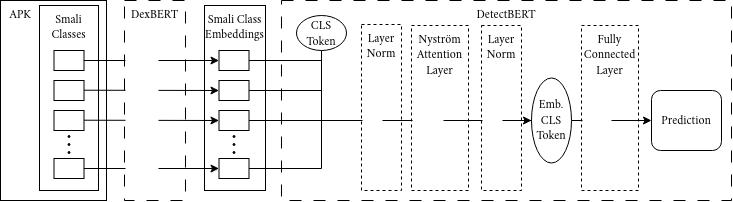
\includegraphics[width=\textwidth]{3_Methodology/detectbert_schema.png}
        \captionsetup{width=\textwidth}
        \caption{\label{fig:detectbert_schema}
        Overview of the DetectBERT architecture. 
        The model processes APK files by extracting small class representations using DexBERT, 
        which generates embeddings for each class. 
        A CLS token is added to the sequence, 
        followed by layer normalization and a Nyström attention layer. 
        Additional layer normalization is applied before feeding the CLS token embedding 
        into a fully connected layer to generate the final prediction.
        }
    \end{minipage}
\end{figure*}


In the previous chapters, various non Transformer based approaches for 
static Android malware detection were explored. 
These methods rely on traditional machine learning techniques and therefore  
struggle with capturing the complex relationships within Android application data. 
In contrast, Transformer based models have demonstrated SOTA 
performance in various NLP and code understanding tasks \cite{transformer_sota}. 
This chapter introduces DetectBERT \cite{detectbert}, the first Transformer-based approach examined 
in this thesis.

DetectBERT is a static Android malware detection model that utilizes Transformer based architectures for analyzing APK files.
Its processing schema is visualized in figure \ref{fig:detectbert_schema}.
Specifically, DetectBERT processes the classes.dex file contained within Android APKs by extracting Smali class representations. 
These representations are subsequently transformed into compact feature embeddings using DexBERT \cite{dexbert}, 
a specialized Transformer model developed by the same authors for this task.
These embeddings serve as inputs to the DetectBERT component, a Transformer architecture that employs Nyström based attention \cite{nystromformer} 
to effectively manage computational complexity while capturing long-range dependencies. 
The embeddings, together with a special CLS token, designed to aggregate global context, are refined through successive layer normalization and Nyström attention layers. 
This processing aims for, global feature representation encapsulated in the embedding of the CLS token.
Finally, DetectBERT uses a fully connected  layer to process the Embedded CLS token into a  malware prediction, indicating whether the APK is malicious or benign.

To evaluate DetectBERT, we benchmarked its performance on the DexRay ad Transcend datasets. 
Due to computational and time constraints, the full DexRay and Transcend datasets were not used. 
Instead, subsets of both datasets were generated, each containing 20,000 APKs with an even label distribution. 
Additionally, the Smali class distributions were balanced between malware and 
goodware samples, countering the inherent imbalance of the DexRay dataset. 
The DexRay dataset is also the dataset that was used for benchmarking the model 
in its original paper. However, due to the Smali class imbalance between labels, 
the benchmarks presented in the paper were not entirely trustworthy. 
The results on the balanced subset do indicate, that the model does not simply rely 
on the number of Smali classes for predictions but at least to some extent, 
utilizes other information extracted from the Smali class embeddings. 
However, the results on the subsets are not as good as those provided in the 
original paper (see Table \ref{tab:detectbert_performance_original}). 
This performance discrepancy might also be attributed 
to the smaller training dataset size used in our experiments.

The model was tested under two different data splitting strategies: a random split, 
which ensures a balanced distribution of samples in training and testing, 
and a time based split, which simulates realworld conditions by training on older 
data and testing on newer samples. 
Table \ref{tab:detectbert-results} presents the detection performance of DetectBERT across both datasets 
and splits. The results indicate that DetectBERT is
achieving high accuracy and F1 scores, particularly on the DexRay dataset. 
The model demonstrates a slight decline in performance for time-based splits, 
likely due to evolving malware patterns. 
The performance on the subset of the Transend dataset are not as good as 
on the DexRay dataset.

The evaluation gives several key insights about DetectBERTs performance. 
Transformer based models effectively capture complex relationships in APK data, 
surpassing traditional methods for the Transcend dataset (see table \ref{tab:decisiontree30}). 
The DexRay dataset yields better results compared 
to Transcend, suggesting dataset specific challenges. 
The time based split introduces a more realistic evaluation setting, 
exposing the impact of concept drift in malware evolution.

Overall, DetectBERT is implemented as a TransMIL model , which is a Transformer based 
multiple instance learning (MIL) framework \cite{transmil}. 
In this approach, the model processes 
multiple Smali class embeddings as instances within an APK and learns to make a 
classification decision based on the most relevant instances. This allows DetectBERT 
to focus on the most informative Smali class embeddings rather than relying on 
simple aggregate statistics, improving its ability to detect malware patterns effectively.

\begin{margintable}[-30\baselineskip]
    \caption{\label{tab:detectbert_performance_original} DetectBERT Performance Results (accuracy, precision, recall, F1 Score) from the original paper \cite{detectbert}}
    \footnotesize
    \begin{tabular*}{\linewidth}{@{\extracolsep{\fill}} cccc@{}}
        \toprule
        \textbf{Acc.} & \textbf{Prec.} & \textbf{Rec.} & \textbf{F1} \\
        \midrule
        97\% & 98\% & 95\% & 97\% \\
        \bottomrule
    \end{tabular*}
\end{margintable}




\begin{table}[]
    \caption{\label{tab:detectbert-results}%
        DetectBERT Benchmark Results Across Datasets and Splits.  
        The results are reported for both random and time-based splits, 
        highlighting the effectiveness of the model in distinguishing between 
        goodware and malware. 
        On the DexRay dataset, DetectBERT consistently achieves higher accuracy, 
        particularly for goodware classification.}
    \resizebox{\textwidth}{!}{%
    \begin{tabular}{@{}llcccc@{}}
    \toprule
    \textbf{Dataset} & \textbf{Split} & \textbf{Accuracy} & \textbf{Precision} & \textbf{Recall} & \textbf{F1} \\ \cmidrule(r){1-2} \cmidrule(lr){3-6}
    DexRay (Subset)  & Random     & 89.57\% & 89.57\% & 89.57\% & 89.57\% \\
                     & Time-based & 89.17\% & 90.00\% & 89.17\% & 89.10\% \\ \addlinespace
    Transcend (Subset) & Random     & 81.77\% & 82.46\% & 81.77\% & 81.77\% \\
                       & Time-based & 78.67\% & 78.73\% & 78.67\% & 78.68\% \\
    \bottomrule
    \end{tabular}%
    }
\end{table}

\newpage

\section{Experimntal Setup}

\subsection{General BERT based approach}

\begin{figure*}[b]
    \centering
    \begin{minipage}{1.5\textwidth}
        \centering
        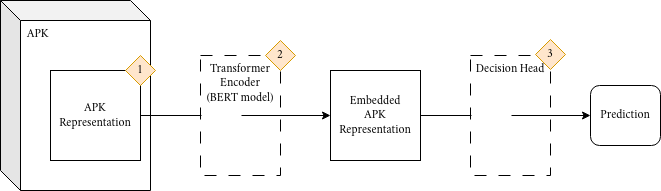
\includegraphics[width=\textwidth]{3_Methodology/bertbased_malwaredetection_schema.png}
        \captionsetup{width=\textwidth}
        \caption{\label{fig:bertbased_malwaredetection_schema}
        Generalized BERT-based approach for malware detection. 
        This figure illustrates a blueprint for utilizing BERT models in APK-based 
        malware detection. 
        The process consists of three main stages: 
        extracting an APK representation [1], 
        encoding it using a Transformer based model (BERT) [2], 
        and applying a decision head to generate the final prediction [3]. 
        The numbered elements indicate open design choices within this blueprint.
        }
    \end{minipage}
\end{figure*}

The experiments conducted in this thesis build upon a generalized paradigm 
for malware detection, as visualized 
in figure \ref{fig:bertbased_malwaredetection_schema}. 
The core idea is that, in order to classify an APK as malicious or benign, 
it must first be processed through a structured pipeline.

The first step [1] involves extracting an appropriate representation of the APK. 
This representation serves as the input for the subsequent stages 
and can be derived from different static attributes of the APK, 
ensuring that relevant structural and behavioral information is preserved.

Next, in step [2], this representation undergoes an embedding process. 
The embedding is designed to transform the extracted representation into 
a format suitable for processing further while maintaining essential 
information and reducing dimensionality. 
The choice of embedding strategy significantly influences the quality 
of the learned representation and consequently, the detection performance.

In the final step [3], the embedded representation is passed to a 
decision head that generates the final classification. 
The decision head can take various forms, from simple fully connected layers
to more complex Transformer based network structures. 
The effectiveness of the decision head plays a crucial role in 
ensuring that the model correctly distinguishes between benign 
and malicious applications.

The objective of this thesis is to analyze the capabilities of 
this architecture by systematically evaluating each of these three 
core components. By designing experiments that focus on variations 
in APK representation, embedding methods, and decision heads, 
the study aims to provide insights into the strengths and limitations 
of Transformer based malware detection models. 
The following chapters will further explore each of these stages in detail, 
discussing alternative design choices and their impact on detection performance.
